\def \currentAuthor {Gabi Sorglos} %so kann jederzeit der Autor geändert werden -> wird in der Fusszeile angezeigt.

\chapter*{Einleitende Bemerkungen}

\chapter*{Notationen}
Beschreibung wie Code, Hinweise, Zitate etc. formatiert werden  

\chapter{Projektmanagement}

\section{Metainformationen}
\subsection{Team}
Christopher Haider (Leiter, Programmierer, Design), Maximilian Egger (Programmierer, Druck)
\subsection{Betreuer}
NEUNER Dominik, MSc
\subsection{Partner}
HAK Imst
\subsection{Ansprechpartner}
NEUNER Dominik, MSc
\section{Vorerhebungen}
\subsection{Projektzieleplan}

\textbf {-Einteilung:}


\textbf {OBERZIEL} Es soll eine Applikation entwickelt werden, bei der Fragen (zu einem Thema) und zugehörigen mögliche Antworten (mit einer richtigen) erstellt werden können. Jeder Frage muss ein Standort auf der Karte zugewiesen werden.
Im Front-End können Fragen im Umkreis aufgelistet und gelöst werden. Für jede gelöste Frage erhöht sich der Punktestand des Benutzers.  


\textbf {LEISTUNGSZIEL} Das Projekt wird mehrere Mitarbeiter beinhalten und wir versuchen den einzelnen Mitarbeitern die optimale Arbeit zuzuweisen, um eine pünktliche Fertigstellung mit würdiger Qualität zu erreichen. Implementierung von aktuellen Karten und Standort, kleine Übersicht des Punktestandes, Backend/Frontend;


\textbf {KOSTENZIEL} Die Kosten belaufen sich ca. in Höhe von 8.500 - 12.500 € abhängig von der Zeit der aktiven Arbeit jedes einzelnen Mitarbeiters/Programmierer plus den Überstunden inklusive allen Aufwänden für die Programmierung, Serverwartungen, laufende Aktualisierungen von den Daten. Abgesehen von den Steuern.


\textbf {TERMINZIEL} Dieses etwas umfangreichere Projekt sollte mit Einplanung vom 14.03.2017 in einem Zeitrahmen bis Ende November/Dezember in Form von einer kompakten App im Store verfügbar sein.


\textbf {DETAILZIEL} Unserem Partner/Kunden vor der endgültigen Fertigstellung des Projekts eine Testapp /  Prototypapp vorzeigen und nochmals eine endgültige Absprache mit den Kunden abhalten.



\subsection{Projektumfeld}

\begin{figure}
	\centering
	\includegraphics[width=1\linewidth]{../Grafik1}
	\caption{Projektnähe tabellarisch}
	\label{fig:grafik1}
\end{figure}


\begin{figure}
	\centering
	\includegraphics[width=1\linewidth]{../Grafik}
	\caption{Projektnähe Grafisch}
	\label{fig:grafik}
\end{figure}




Welche Bedrohungen bestehen für das Projekt
Budget Überschreitung
\begin{itemize}
	\item Termine nicht einhalten
	\item Auftragsgeber sagt ab
	\item Auftragsgeber ändert seine Anforderungen
	\item Probleme bei der Realisierung
\end{itemize}



\subsection{Risikoanalyse}
\begin{figure}
	\centering
	\includegraphics[width=1.2\linewidth]{../Grafik2}
	\caption{Risikomatrix}
	\label{fig:grafik2}
\end{figure}

\section{Pflichtenheft}
\subsection{Zielbestimmung}

\textbf {Projektbeschreibung}
 Es soll eine Applikation entwickelt werden, bei der Fragen (zu einem Thema) und zugehörigen mögliche Antworten (mit einer richtigen) erstellt werden können. Jeder Frage muss ein Standort auf der Karte zugewiesen werden.
Im Front-End können Fragen im Umkreis aufgelistet und gelöst werden. Für jede gelöste Frage erhöht sich der Punktestand des Benutzers.

\textbf {IST-Zustand}
Diese Applikation gibt es nach dieser Weise noch nicht, dennoch sind Ähnlichkeiten mit Pokemon Go zu erkennen. Obwohl es nicht um Pokemon geht, sonder um Fragen und Antworten die einen Standort besitzen.

\textbf {SOLL-Zustand}
Diese Applikation soll dem Nutzer die Möglichkeit geben Informatik außerhalb des Gebäudes zu beantworten. Dies soll die Anwender anregen mehr ins freie zu gehen um Sport zu betreiben, dennoch sein Wissen im Bereich IT zu erweitern


\subsection{Produkteinsatz und Umgebung}
\begin{itemize}
	\item in Form einer App im Store erhältlich
	\item Jugendliche und Erwachsene
	\item Lizenz
	\item GPS, Android-Phone und Internetverbindung
\end{itemize}
\subsection{Funktionalitäten}
\begin{itemize}
	\item MUSS-Anforderungen
	\begin{itemize}
		\item Fragen hinzufügen, Antworten hinzufügen, Punktestand erhöhen, Standort muss sich ändern können, Absturz der App vermeiden
		\item Design, auf allen Plattformen erhältlich
	\end{itemize}
	\item KANN-Anforderungen
	\begin{itemize}
		\item Fehlerausgabe, 
		\item Nicht-funktional
	\end{itemize}
\end{itemize}
\subsection{Testszenarien und Testfälle}
\begin{itemize}
	\item Beschreibung der Testmethodik
	\item Testfall 1
	\item Testfall 2
	\item \ldots
\end{itemize}
\subsection{Liefervereinbarung}
\begin{itemize}
	\item Applikation
	\item Adminmodus, Benutzermodus
	\item Designer, Programmierer, Web-Designer
\end{itemize}
\section{Planung}
\subsection{Projektstrukturplan}


\begin{itemize}
	\item Verteilung der Arbeit
	\item Gerechte Arbeitsaufteilung bzw. Gehalt
	\item Ausführung des Projekts
	\item Kontrolle (Funktional- und Qualitätskontrolle)
	\item Testdurchlauf (Prototyp)
	\item Möglich Fehler beheben bzw. dem Kunden präsentieren
\end{itemize}

\subsection{Meilensteine}
Einteilung in Etappen = sogenannte Zwischenziele, erleichtert die Projektplanung


\begin{itemize}
	\item Einteilung
	\item Ausführung
	\item Kontrolle
	\item Testdurchlauf
	\item Endprodukt
\end{itemize}



\subsection{Gant-Chart}

\begin{figure}
	\centering
	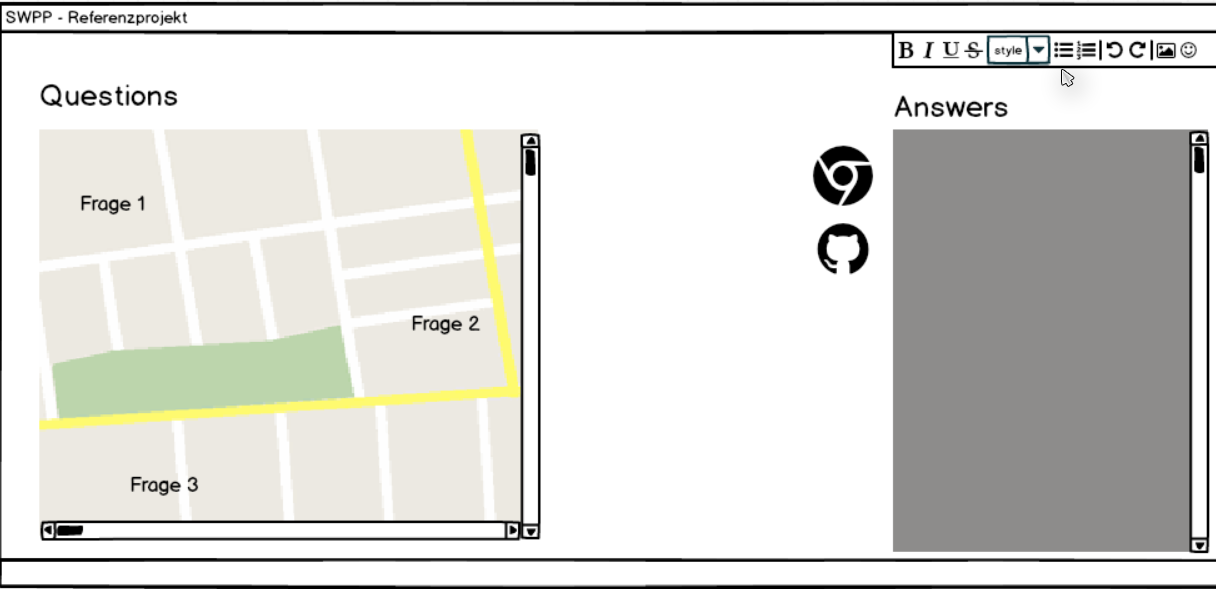
\includegraphics[width=1.8\linewidth]{screenshot002}
	\caption{}
	\label{fig:screenshot002}
\end{figure}


\subsection{Abnahmekriterien}


= Bezeichnung des letzten Schritts in der Systemauswahl
Erfolgt nach erfolgreich, abgeschlossenen Projektbetrieb.

Umfasst Hard- und Softwarekomponenten -> Berücksichtigung der Leistungsanforderungen

\textbf {natürlichsprachliches abstraktes Abnahmekriterium}

Ausgangssituation:
Mindestens 1 Nutzer ist in der App (virtuellen Welt) angemeldet

Ereignis:
Im Rahmen des Spielvorgangs der App kann der Nutzer seinen Charakter auswählen und sich auf die virtuelle Map begeben

erwartetes Ergebnis:
der Nutzer kann ohne Probleme auf der Map umhergehen und gestellte IT-Fragen beantworten in Form einer spielerischen Art


\textbf {formalisiert abstraktes Abnahmekriterium}

In Form einer Tabelle

Ablauf:

\begin{itemize}
	\item Nutzer hat die volle Kontrolle über seinen eigenen Charakter in der App bzw. Webseite

	\item Er kann seinen Charakter bearbeiten und PlugIns importieren, Mapskins und weitere Layoutänderung in der App vornehmen die       keinen Einfluss auf die Funktionalität haben
		
	\item Ihm wird ermöglicht Fehlerquellen beheben zu können 

	\item Bildschrimausgabe auf dem Screen des Nutzers
	
	\item Seine Ergebnisse der beantworteten Fragen können online
	gespeichert oder lokal ausgedruckt werden -> Rangliste 
		 
\end{itemize}

\subsection{Pläne zur Evaluierung}


Wesentlich für seriöse und erfolgreiche (Selbst-)Evaluation sind vor allem …



\textbf {einsichtige Gründe und spürbare Folgen}
\begin{itemize}
		\item erweitern des Wissens in der Natur indem man zu Standorten auf der App läuft/geht und eine Frage beantwortet oder eine Frage erstellt
	\end{itemize}




\textbf {ein positiver Ansatz}

\begin{itemize}
		\item einzigartig, aktuell, qualitativ hochwertig, Benutzerfreundlich
\end{itemize}




\textbf {relevante Fragestellungen und Kriterien}

\begin{itemize}
		\item möglichst viel Aufmerksamkeit der User bekommen
		\item Bekanntheitsgrad erhöhen
		\item Feedback von den Usern zur App bekommen
	\end{itemize}




\textbf {wirksame Methoden und Instrumente}

\begin{itemize}
		\item App ist völlig Kostenlos
		\item leicht bedienbar
		\item für jede Altersklasse tauglich
\end{itemize}


\textbf {ein multiperspektivischer Ansatz}

Da unser Professor sich diese Applikation zunächst auf Fehler bzw. Macken analysiert und wir sie dann der Klasse vorstellen werden  wir uns wahrscheinlich die ein oder andere Idee noch einbauen oder einen Prototypen erstellen bevor wir es im Markt präsentieren.

\textbf {klare Verantwortlichkeiten und Entscheidungsstrukturen}


Verantwortlich für Projekt/App bzw. Webseite sind wir selbst. (Christopher Haider und Maximilian)
Entscheidungen werden nur durch Christopher Haider den Projektleiter zustande kommen.
Mehr Informationen zu den jeweiligen Themen finden Sie oben bei der Abbildung 1.6.


\textbf {machbare Pläne und gesicherte Rahmenbedingungen}

Qualifikationen: Beteiligte dieses Projektes besitzen spezielle Fachkenntnisse bzw. Qualifikationen

Zeit: Unser Plan ist es dieses Projekt bis Ende Schulschluss fertigzustellen.

Geldmittel: 


\subsection{Ergänzungen und zu klärende Punkte}


\chapter{Vorstellung des Produktes}
Vorstellung des fertigen Produktes anhand von Screenshots, Bildern, Erklärungen.

\chapter{Eingesetzte Technologien}
\begin{itemize}
	\item html, java script, php, datenbank (sql), css
	\item php, html, css, java script, datenbank
	\item ajax
	\item css
\end{itemize}

\chapter{Problemanalyse}
\section{USE-Case-Analyse}
\begin{itemize}
	\item UseCases auf Basis von Benutzerzielen identifizieren: 
	\begin{itemize}
		\item Benutzer eines Systems identifizieren
		\item Benutzerziele identifizieren (Interviews)
		\item Use-Case-Liste pro Benutzer definieren
	\end{itemize}
	\item UseCases auf Basis von Ereignissen identifizieren: 
	\begin{itemize}
		\item Externes Event triggert einen Prozess
		\item zeitliches Event triggert einen Prozess (Zeitpunkt wird erreicht) 
		\item State-Event (Zustandsänderung im System triggert einen Prozess)
	\end{itemize}
	\item Werkzeuge:
	\begin{itemize}
		\item USE-Case-Beschreibungen (textuell, tabellarisch)
		\item USE-Case-Diagramm
		\item Aktivitätsdiagramm für den Use-Case (Interaktion zwischen Akteur und System abbilden)
		\item System-Sequenzdiagramm (Spezialfall eines Sequenzdiagramms: Nur 1 Akteur und 1 Objekt, das Objekt ist das komplette System, es geht um die Input/Output Requirements, die abzubilden sind)
	\end{itemize}
\end{itemize}

\section{Domain-Class-Modelling}
\begin{itemize}
	\item "Dinge" (Rollen, Einheiten, Geräte, Events etc.) identifizieren, um die es im Projekt geht
	\item ER-Modellierung oder Klassendiagramme
	\item Zustandsdiagramme (zur Darstellung des Lebenszyklus von Domain-Klassen darstellen)
\end{itemize}

\section{User-Interface-Design}
\begin{itemize}
	\item Mockups
	\item Wireframes
\end{itemize}


\chapter{Systementwurf}

\section{Architektur}

\subsection{Design der Komponenten}

Darstellung und Beschreibung der Systemarchitektur;

\begin{itemize}
	\item  statische Zerlegung des Systems in seine physischen Bestandteile (Komponenten, Komponentendiagramm)
	\item (textuelle) Beschreibung des dynamischen Zusammenwirkens aller Komponenten 
	\item (textuelle) Beschreibung der Strategie für die Architektur, d. h. wie die Architektur in Statik und Dynamik funktionieren soll.
	\item Verwendung von Referenzarchitekturen bzw. Architekturmustern (als Schablonen, z.B. MVC. Plugin, Pipes and Filters)
	\begin{itemize}
		\item MVC
		\item Schichten
		\item Pipes
		\item Request Broker
		\item Service-Oriented
	\end{itemize}
\end{itemize}

\subsection{Benutzerschnittstellen} 
\begin{itemize}
	\item Design des UIs
	\item Dialoge, Dialogsteuerung, Ergonomie, Gestaltung, Eingabeüberprüfungen
\end{itemize}

\subsection{Datenhaltunskonzept}
\begin{itemize}
	\item Design der Datenbank (ER-Modell)
	\item Design des Zugriffs auf diese Daten (Datenhaltungskonzept)
	\item Caching, Transaktionen
\end{itemize}

\subsection{Konzept für Ausnahmebehandlung}
\begin{itemize}
	\item Systemweite Festlegung, wie mit Exceptions umgegangen wird
	\item Exceptions sind primär aus den Bereichen UI, Persistenz, Workflow-Management
\end{itemize}

\subsection{Sicherheitskonzept}
Beschreibung aller sicherheitsrelevanten Designentscheidungen

\begin{itemize}
	\item Design der Security-Elemente
	\item Design von Safety-Elementen (Fehlertoleranz, Verfügbarkeit etc.)
\end{itemize}

\subsection{Design der Testumgebung}
\begin{itemize}
	\item wie wird getestet (Unit-Testing, Integrationstesting, Systemtests, Akzeptanztests)
	\item Testumgebung, Testprozess, Teststrategie, Testmethoden, Testfälle
\end{itemize}


\subsection{Desing der Ausführungsumgebung}
\begin{itemize}
	\item Deployment (DevOps)
	\item Betrieb (besonders Hoch- und Hertunerfahren der Anwendung)
\end{itemize}

\section{Detailentwurf}

Design jedes einzelnen USE-Cases

\begin{itemize}
	\item Design-Klassendiagramme vom Domain-Klassendiagramm ableiten (incl. detaillierter Darstellung und Verwendung von Vererbungshierarchichen, abstrakten Klassen, Interfaces)
	\item Sequenzdiagramme vom System-Sequenz-Diagramm ableiten
	\item Aktivitätsdiagramme
	\item Detaillierte Zustandsdiagramme für wichtige Klassen
\end{itemize}

Verwendung von CRC-Cards (Class, Responsibilities, Collaboration) für die Klassen
\begin{itemize}
	\item um Verantwortlichkeiten und Zusammenarbeit zwischen Klassen zu definieren und
	\item um auf den Entwurf der Geschäftslogik zu fokussieren
\end{itemize}

Design-Klassen für jeden einzelnen USE-Case können z.B. sein:

\begin{itemize}
	\item UI-Klassen
	\item Data-Access-Klassen
	\item Entity-Klassen (Domain-Klassen)
	\item Controller-Klassen
	\item Business-Logik-Klassen
	\item View-Klassen
\end{itemize}

Optimierung des Entwurfs (Modularisierung, Erweiterbarkeit, Lesbarkeit):

\begin{itemize}
	\item Kopplung optimieren
	\item Kohäsion optimieren
	\item SOLID
	\item Entwurfsmuster einsetzen
\end{itemize}

\chapter{Implementierung}
Detaillierte Beschreibung der Implementierung aller Teilkomponenten der Software entlang der zentralsten Use-Cases:

\begin{itemize}
	\item GUI-Implementierung
	\item Controllerlogik
	\item Geschäftslogik
	\item Datenbankzugriffe
\end{itemize}

Detaillierte Beschreibung der Teststrategie (Testdriven Development):

\begin{itemize}
	\item UNIT-Tests (Funktional)
	\item Integrationstests
\end{itemize}

Zu Codesequenzen:
\begin{itemize}
	\item kurze Codesequenzen direkt im Text (mit Zeilnnummern auf die man in der Beschreibung verweisen kann)
	\item lange Codesequenzen in den Anhang (mit Zeilennummer) und darauf verweisen (wie z.B. hier \cref{qj})
\end{itemize}

\chapter{Deployment}
\begin{itemize}
	\item Umsetzung der Ausführungsumgebung
	\item Deployment
	\item DevOps-Thema
\end{itemize}

\chapter{Tests}

\section{Systemtests} 
Systemtests aller implementierten Funktionalitäten lt. Pflichtenheft
\begin{itemize}
	\item Beschreibung der Teststrategie
	\item Testfall 1
	\item Testfall 2
	\item Tesfall 3
	\item …
\end{itemize}

\section{Akzeptanztests}

\chapter{Projektevaluation}
siehe Projektmanagement-Unterricht

\chapter{Benutzerhandbuch} 
falls im Projekt gefordert

\chapter{Betriebswirtschaftlicher Kontext}
BW-Teil

\chapter{Zusammenfassung}
\begin{itemize}
	\item Etwas längere Form des Abstracts
	\item Detaillierte Beschreibung des Outputs der Arbeit
\end{itemize}